\documentclass[12pt,prb,aps,epsf]{report}
\usepackage[utf8]{inputenc}
\usepackage{amsmath}
\usepackage{amsfonts}
\usepackage{amssymb}
\usepackage{graphicx} 
\usepackage{latexsym} 
\usepackage[toc,page]{appendix}
\usepackage{listings}
\usepackage{xcolor}
\usepackage{soul}
\usepackage[T1]{fontenc}
\usepackage{amsthm}
\usepackage{mathtools}
\usepackage{setspace}
\usepackage{array,multirow,makecell}
\usepackage{geometry}
\usepackage{textcomp}
\usepackage{float}
%\usepackage{siunitx}
\usepackage{cancel}
%\usepackage{tikz}
%\usetikzlibrary{calc, shapes, backgrounds, arrows, decorations.pathmorphing, positioning, fit, petri, tikzmark}
\usepackage{here}
\usepackage{titlesec}
%\usepackage{bm}
\usepackage{bbold}

\geometry{hmargin=2cm,vmargin=2cm}

\begin{document}
	
	\title{MP 24 Signal et bruit}
	\author{Naïmo Davier}
	
	\maketitle
	
	\tableofcontents
	
	\pagebreak
	
	
\paragraph{Signal :} Un signal est une information codée dans le but d'être transmise, depuis un émetteur vers un récepteur.
\paragraph{Bruit :} Le bruit représente toutes les informations décorrélées avec le signal d'intérêt et qui viennent par conséquent perturber la lecture de l'information lors de la réception.

\section{Caractérisation d'un bruit de quantification}
On veut dans cette partie caractériser le bruit de quantification dû à la numérisation d'un signal en regardant l'impact d'un échantillonneur bloqueur sur un signal donné.\\

\begin{figure}[h]
	\centerline{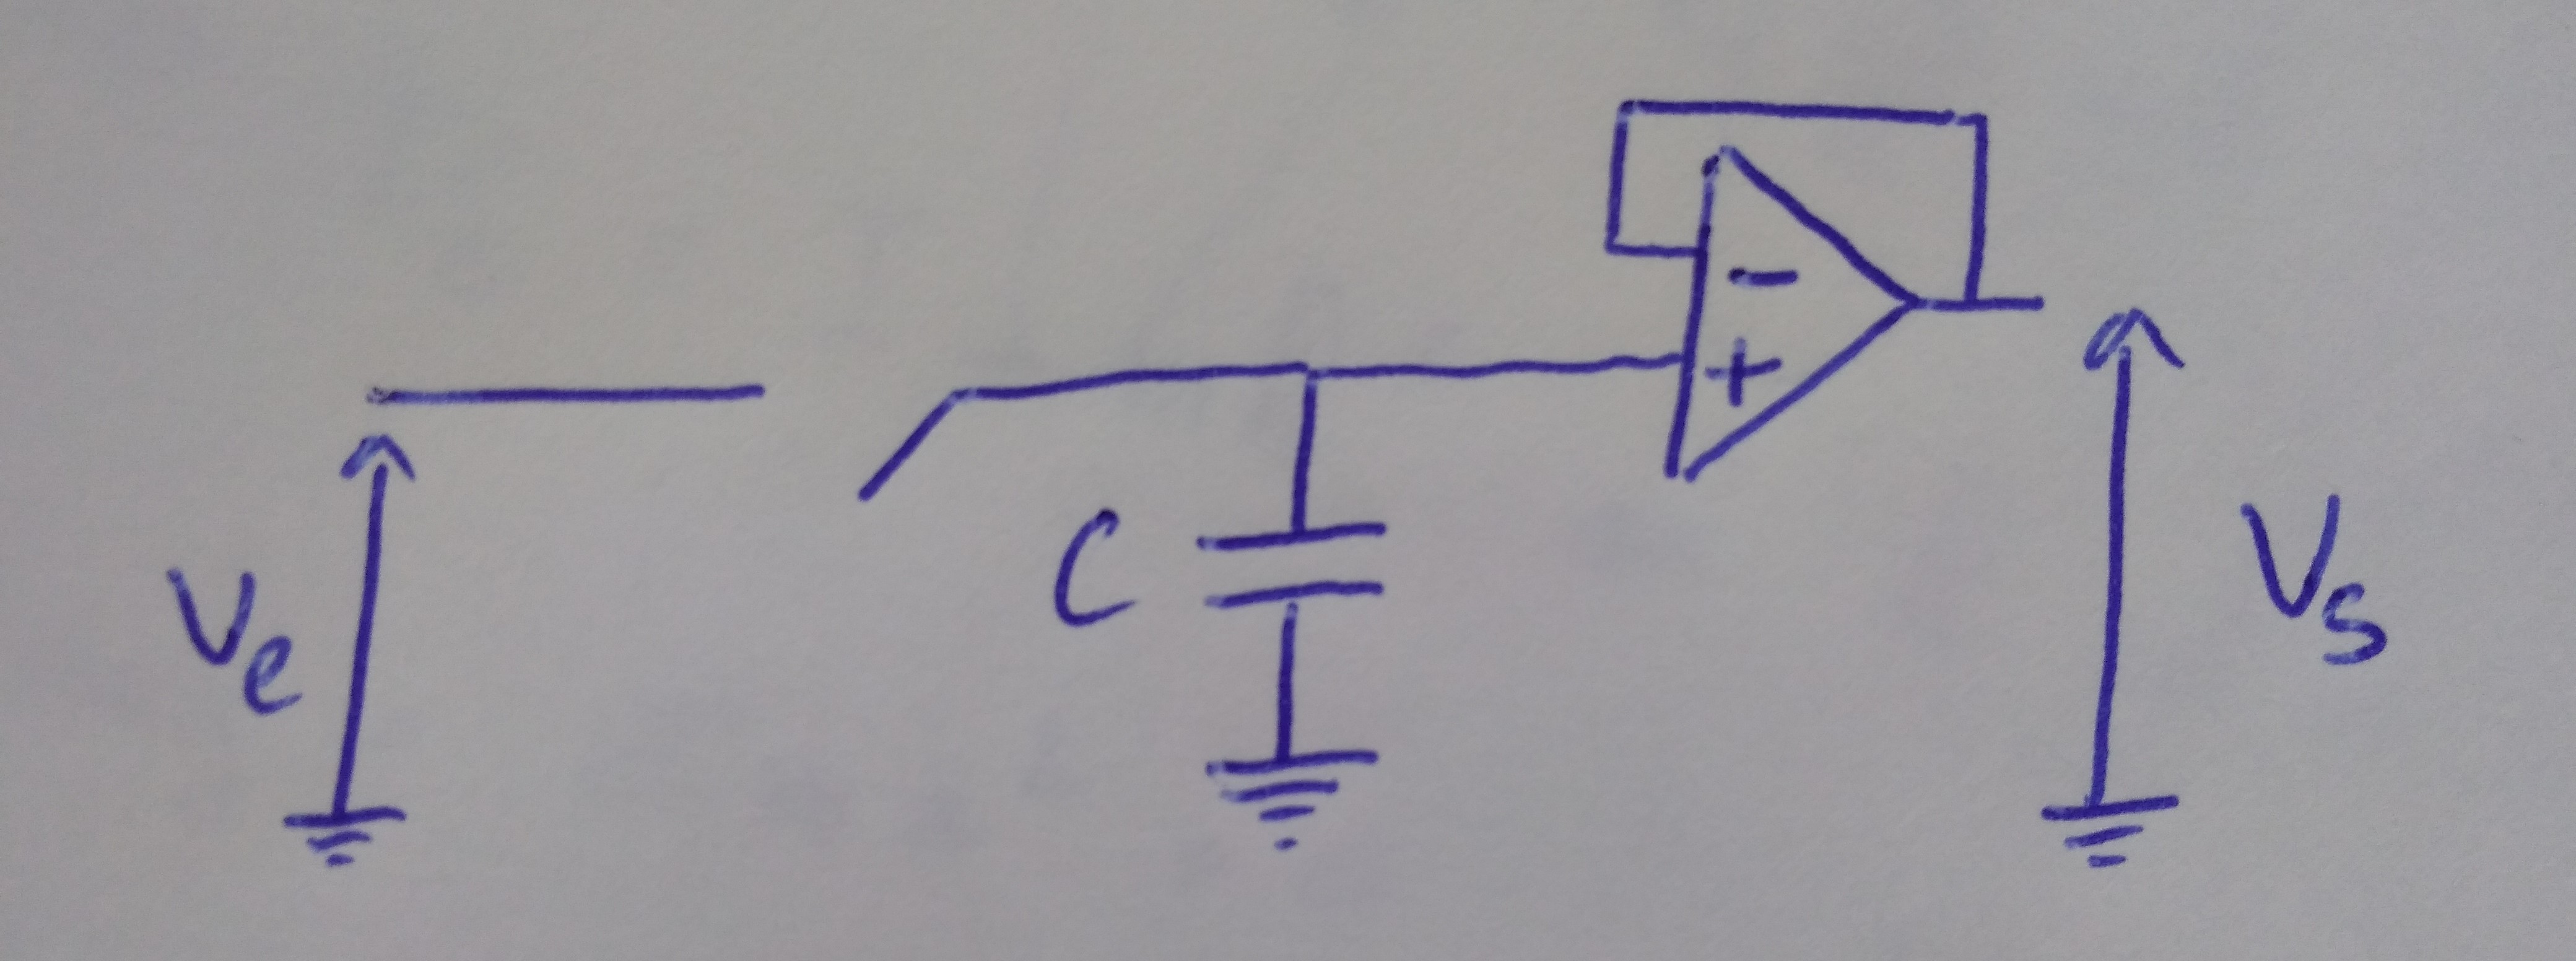
\includegraphics[width=11cm]{P1S1}}
\end{figure}

On utilise ici un échantillonneur-bloqueur constitué par un interrupteur géré par la sortie TTL d'un GBF, faisant office d'horloge, d'une capacité $C$ et d'un suiveur.

La valeur de la capacité $C$ du condensateur doit être ici minimale pour avoir un temps d'acquisition $T_{acq}$ minimum, ce dernier correspondant au minimum à son temps de charge $\tau \sim R_{interrupteur}C$. Cependant l'AO n'étant en réalité pas idéal il y a un léger courant $i_0$ au niveau de sa borne +, conduisant à une décharge du condensateur en un temps $\tau_d$ de l'ordre de $\frac{C}{i_0}$ car 
\begin{eqnarray}
i_0 = -C\frac{dV}{dt}\; \Rightarrow \; V(t) = V_0 - \int_0^t \frac{i_0}{C}\,ds = V_0-\frac{i_0}{C} t
\end{eqnarray} 
ce qui limite donc la valeur de $C$ qui doit être suffisamment grande pour que $\tau_d \gg T_{acq}$.\\
Ici pour la maquette donnée on a $R_{interrupteur}\sim 100 \Omega$ et on prend donc $C = 4,7nF$ (on trouve le C optimal en testant).\\
\paragraph{Remarque :} Si la fréquence du signal d'entrée $f$ est trop grande alors le maximum de sa dérivée $\max(\frac{dV_e}{dt}) = 2\pi f_0$ est trop élevé pour que le condensateur ait le temps de se charger en un temps $T_{acq}$ et $V_s$ devient alors très différent de $V_e$.
\begin{figure}[h]
	\centerline{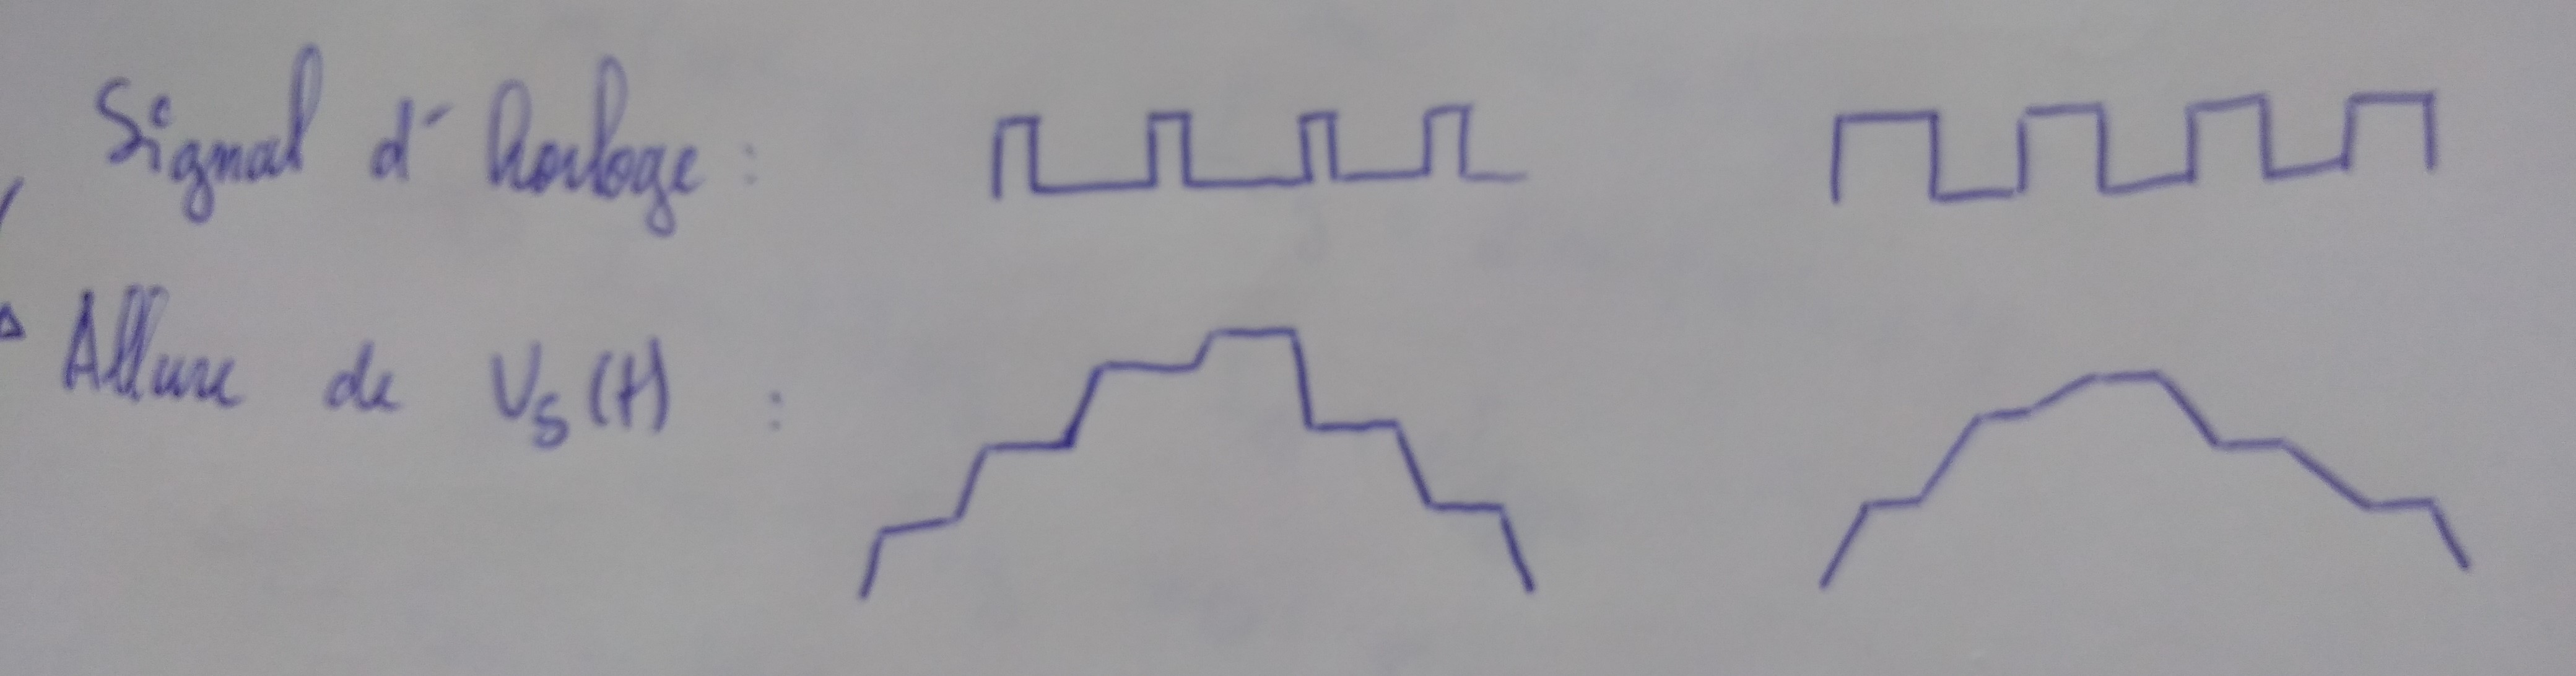
\includegraphics[width=14cm]{P1S2}}
\end{figure}
\paragraph{Remarque} Si on veut un signal qui ressemble bien à un signal numérisé (plats et verticales uniquement) alors il faut prendre un signal d'horloge très asymétrique.\\

On mesure $V_e(t)$ et $V_s(t)$ avec Latis-pro et on en déduit $D(t) = V_e-V_s$. On prend un signal $V_e$ avec une amplitude constante $\rightarrow V_e^{eff}=cste$ et une fréquence $f_0=100 \,Hz$. On fait ensuite varier la fréquence d'échantillonnage $f_e$, on calcule la valeur efficace de D puis on trace le rapport 
\begin{eqnarray}
\gamma = \frac{D^{eff}}{V_e^{eff}}(f_e)
\end{eqnarray}
On trouve en traçant $\ln\gamma (\ln f_e)$ que
\begin{eqnarray}
\gamma = \frac{D^{eff}}{V_e^{eff}}(fe) = \alpha f_e^{-0.85\pm0.05}  \simeq  \frac{\alpha}{f_e}
\end{eqnarray}
On peut expliquer ce résultat : la pente maximale du signal vaut $\beta = 2\pi f_0$, l'écart maximal entre $V_e$ et $V_s$ vaut donc $\beta T_e$, l'écart type sera donc environ proportionnel à $T_e=\frac{1}{f_e}$.

\subsubsection{Rapport signal sur bruit}
Dans la pratique, il serait plus "conventionnel" de mesurer ici le rapport signal sur bruit, qui est le rapport de la puissance de bruit sur la puissance du signal d'entrée
\begin{eqnarray}
RsB = \frac{P_{signal}}{P_{bruit}} = \left(\frac{D^{eff}}{V_e^{eff}}\right)^2
\end{eqnarray}
qu'il convient de donner en décibel, afin d'avoir une comparaison avec des valeurs usuelles de rapport signal sur bruit,
\begin{eqnarray}
RsB_{dB} = 10\log\left(RsB\right) = 10\log\left(\left(\frac{D^{eff}}{V_e^{eff}}\right)^2\right) = 20\log\left(\frac{D^{eff}}{V_e^{eff}}\right)
\end{eqnarray}
On a en effet :\\
$RsB_{dB} \simeq 10\,dB$ pour de la radio\\
$RsB_{dB} \simeq 40\,dB$ pour de l'audio de qualité moyenne (télé, son d'un ordinateur...)\\
$RsB_{dB} \simeq 80-10\,dB$ pour de la hifi, selon la qualité.

\section{Détection synchrone}
Le but du concept de la détection synchrone est de translater la fréquence du signal que l'on veut transmettre dans un domaine de fréquences plus élevé, où le bruit est moindre. On peut ainsi récupérer un signal peu bruité.\\
Idée :\\
- On multiplie le signal que l'on veut transmettre de fréquence $f_0$ par une porteuse de fréquence $f_p \gg f_0$, on obtient ainsi un signal comportant deux fréquences $f_p+f_0$ et $f_p-f_0$ toutes deux grandes devant $f_0$.\\
- On transmet ensuite le signal via une diode ou une antenne dans un milieu pollué par un bruit à basse fréquence.\\
- On re-multiplie notre signal par la porteuse et on obtient ainsi un signal comportant les fréquences $f_0$, $2f_p+f_0$, $2f_p-f_0$...etc.\\
- On applique donc un filtre passe bas permettant de ne garder que $f_0$ : on a ainsi récupéré notre signal initial, modulé par une constante $\alpha$ compliquée à calculer (et dépendant des diodes et de la distance qui les sépare $\rightarrow$ donc pas calculable analytiquement sans sortir une artillerie inadaptée au montage présenté ici).\\
\begin{figure}[h]
	\centerline{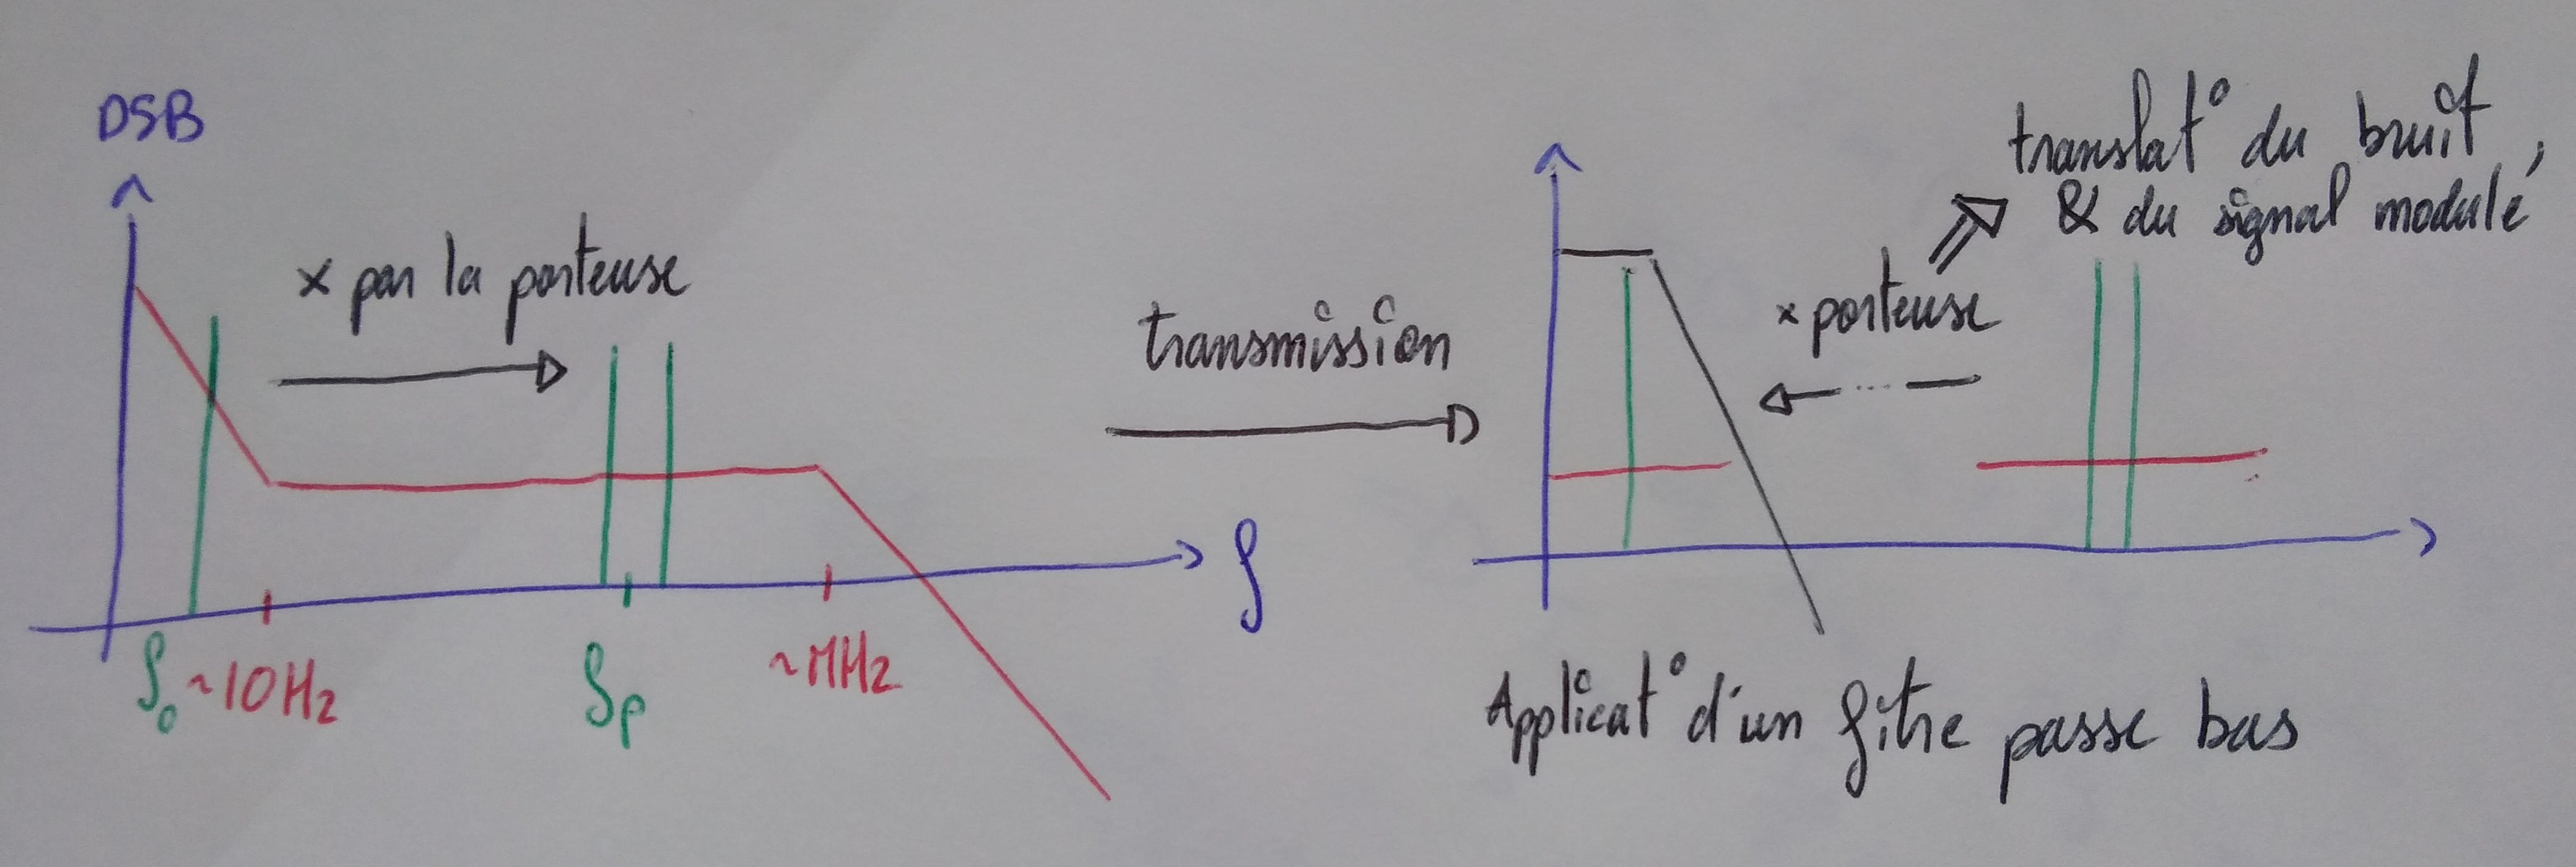
\includegraphics[width=16cm]{P2S1}}
\end{figure}
\begin{figure}
	\centerline{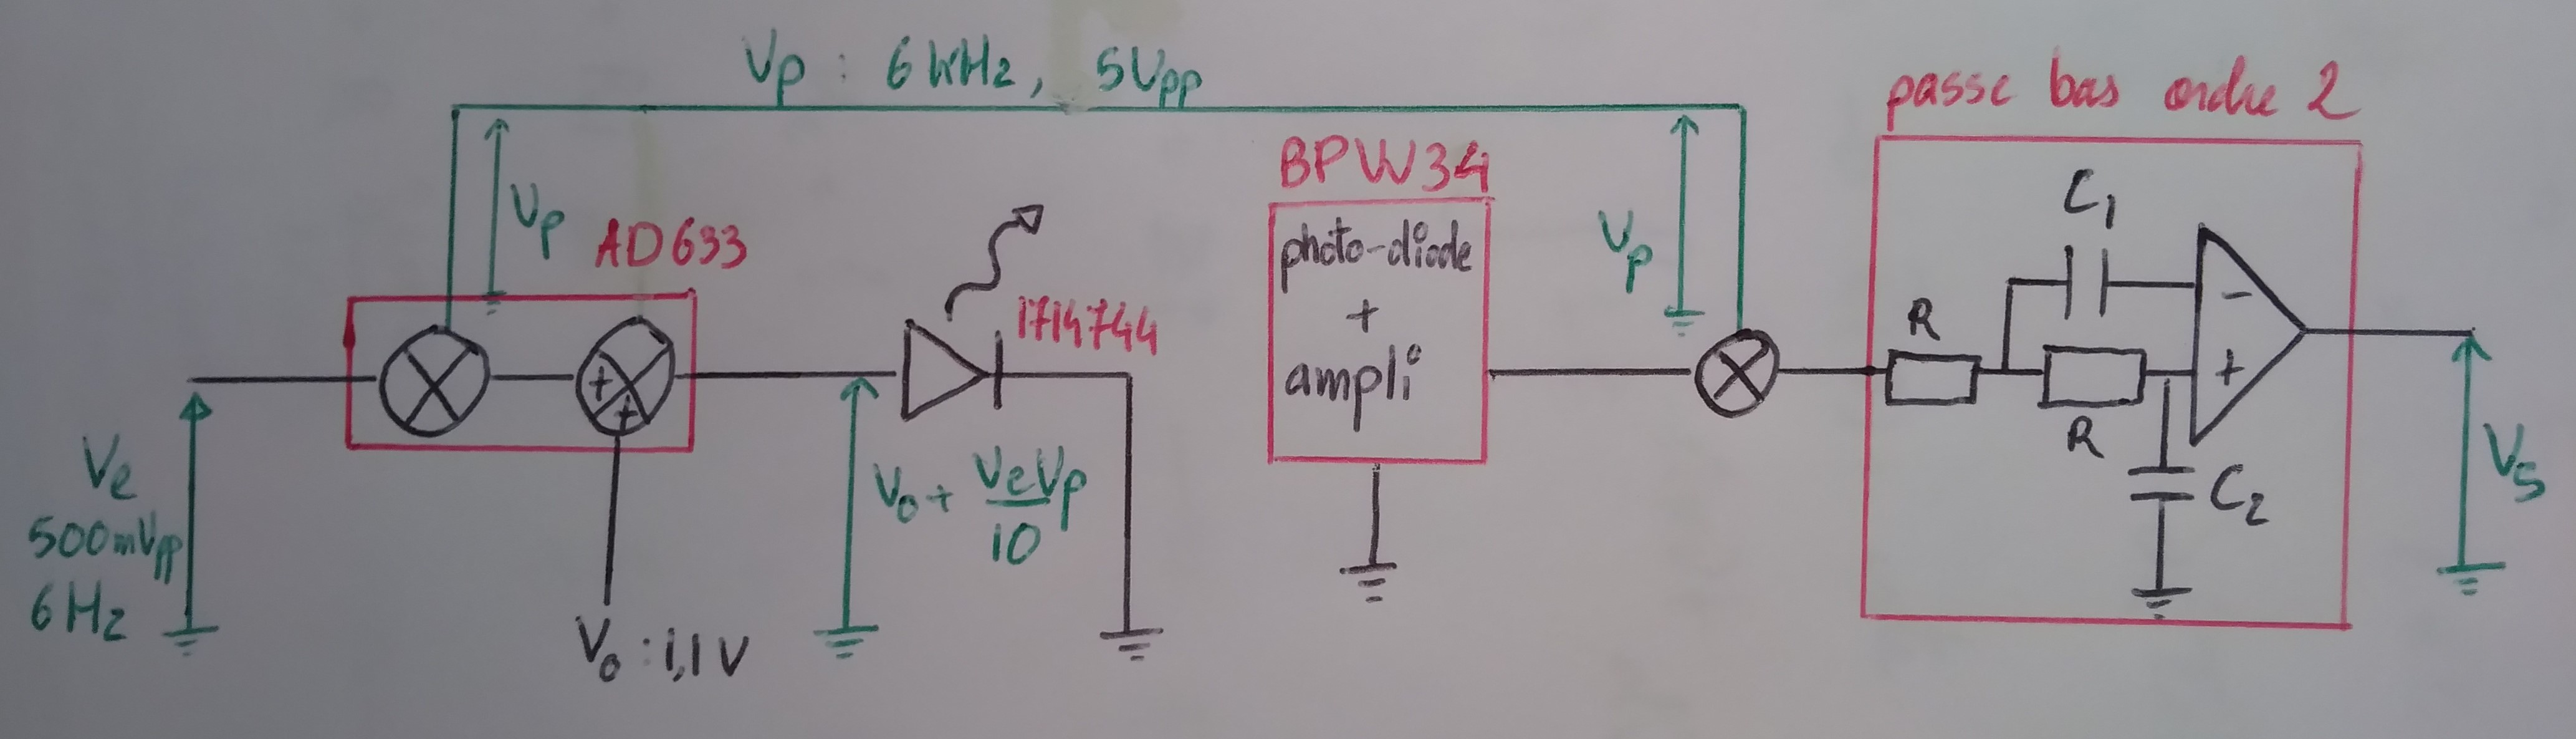
\includegraphics[width=16cm]{P2S2}}
\end{figure}
On réalise ici le montage schématisé ci dessous où l'on transmet le signal via une DEL et où on le reçoit grâce à une photo-diode. Il y a différentes subtilités ici : \\

Si la fréquence de la porteuse $f_p$ est trop élevée la photo diode ne pourra pas réceptionner correctement le signal modulé, car le produit Gain x Bande passante de l'amplificateur en sortie de la BP34 est limité, pour un gain de 100 (ou 10: à vérifier) on observe une bande passante de 8 kHz environ.\\

Il faut appliquer un offset au niveau de la première multiplication afin de placer la DEL dans son régime linéaire, pour l'ensemble donné si dessus on peut voir qu'un offset de $1.1 \,V$ (aux alentours de $1.15\,V$, pas toujours possible à régler précisément : réglable à 0.1V près en général) va bien.\\

Si on construit le passe bas il faudra calculer les valeurs des composantes afin de filtrer entre $f_0$ et $f_p$.\\
Pour le passe bas d'ordre 2 utilisé ici (maquette) on a
\begin{eqnarray}
\omega_c = \frac{1}{RC_1C_2}\hspace{1cm}\&\hspace{1cm} \xi =\sqrt{\frac{C_1}{C_2}}
\end{eqnarray}
Avec $\xi$ le taux d'amortissement que l'on impose à 0.7, ce qui nous fixe le rapport $\frac{C_1}{C_2}$. On a pris ici $f_0=6\,Hz$ et $f_p=6\;kHz$ on cherche donc une fréquence de coupure $f_c \simeq 60\,Hz$, on prend donc 
\begin{eqnarray}
R=21.9\,\Omega,\hspace{0.8cm}C_1=147\,nF, \hspace{0.8cm} C_2=101.6\,nF
\end{eqnarray}
permettant d'avoir $f_c\simeq 59Hz$.\\

Dans ce montage l'essentiel du bruit est celui causé par les néons, qui est à 100Hz (émission de lumière due aux collisions inélastiques entre les atomes du gaz et les électrons porté par le courant électrique à 50Hz délivré par le réseau EDF).\\

Le résultat de cette manipulation sera porté sous la forme d'une comparaison entre le rapport signal sur bruit d'un témoin envoyé sans porteuse et donc ici éclipsé par le bruit à 100Hz, et le rapport signal sur bruit d'une sinusoïde envoyée selon le procédé précédemment décrit.\\ Afin de ne pas effectuer à nouveau qu'un calcul de valeur efficace comme dans le montage précédent, on peut ici regarder, dans le cas où le signal est transmis sans précaution, le spectre de fourrier du signal de sortie et calculer le rapport de l'amplitude de la raie à $6\,Hz$ $A_{6\,Hz}$ sur l'amplitude $A_B$ de la raie à $100\,Hz$ du bruit. \\

Ici on mesure :
\paragraph{Avec détection synchrone}
\begin{eqnarray}
\frac{A_{6Hz}}{\sigma_B} = \frac{28.7\,mV}{0.875\,mV}= 32.8
\end{eqnarray}
\paragraph{En transmettant le signal sans précaution}
\begin{eqnarray}
\frac{A_{6Hz}}{A_B} = \frac{162.3\,mV}{129.4\,mV} = 1.25
\end{eqnarray}
On constate donc bien que la détection synchrone permet ici de limiter le bruit de manière conséquente lors d'une transmission.\\

L'autre point clé de ce montage est qu'il permet de faire un filtre avec un facteur de qualité remarquable. En effet si l'on regarde le processus dans son ensemble il est équivalent à appliquer un filtre passe bande centré à la fréquence $f_p$, or le filtre appliqué en pratique est un filtre passe bas de fréquence de coupure $f_c$ facile à déterminer. Il est de plus possible dans le cas d'un passe bas de réaliser de manière accessible des filtres d'ordre supérieur à 1. Bref l'important est que le facteur de qualité de ce filtre va être égal à 
\begin{eqnarray}
Q = \frac{f_p}{\Delta f} = \frac{f_p}{2f_c}
\end{eqnarray}
où l'on peut choisir $f_p$ et $f_c$, permettant d'obtenir $Q\ll1$. Dans notre cas on a par exemple $f_p=6\,kHz$ et $f_c = 59Hz$ (on utilise un filtre passe bas d'ordre 2 dont l'analyse est faite dans la notice n°10 de la maquette associée) ce qui correspond à $Q \simeq 50$, alors que notre porteuse n'est pas franchement haute fréquence ! Notamment avec des porteuse MHz on obtient des $Q$ supérieurs à $10^4$

\subsection{Remarques pratiques}

La LED a un effet capacitif et se charge donc lorsqu'on y applique la tension que l'on veut transmettre en sortie du premier multiplieur, pour éviter cet effet indésirable qui modifie la tension transmise on peut placer une résistance (de $1k\Omega$ par exemple) entre le multiplieur et la LED afin de limiter le courant et ainsi la charge de la LED.\\

On peut observer un autre effet indésirable lorsque l'on branche la porteuse au second multiplieur : en effet un offset apparait alors sur la tension de sortie du générateur ce qui  le bon goût de "foirer" la première multiplication. Cet effet est néanmoins surmontable en ajoutant un offset arbitraire sur la tension de la porteuse afin de compenser cet offset parasite.

\subsection{questions/remarques}


\end{document} 